\section{Fractal}

フラクタルは数学者ブノワ・マンデルブロが提唱した幾何学の概念である.
自己相似性をもつ図形はどこを拡大しても全体と同じ形を見ることができる.
図はシェルピンスキーのギャスケットと呼ばれるフラクタル図形である.
三角形を一定の法則に基づいて分割していくことで,無限に続いていく三角形が得られる.
その形はどこを拡大しても同様の法則性を持った図形が得られる.
また,自然界の多くの場面でもフラクタル構造をみることができ,自然科学研究の新たなアプローチとしても発展した,

自己相似性を持つ図形はフラクタルという名がつけられる以前から研究されていた.
また,アートとしてもフラクタルを連想するような作品が存在していたが,
コンピュータが普及することによって,様々なフラクタル図形を描画することができるようになり,アートとしても大きく発展した.
この章ではコンピュータで計算,描画されるフラクタルを紹介する.

Fractal Forum\footnote{Fractal Forum:  http://www.fractalforums.com/}では大きなコミュニティが形成されており,多くのフラクタルファンが日夜議論を重ねている.
また,デモシーンという文化でもフラクタルレンダリングとも関連が深い.デモシーンはデモと呼ばれるリアルタイムにCGグラフィクスや音楽を生成するプログラムを見せ合うコンピューターサブカルチャーの一つである.
美しいコンピュータグラフィクスを効率よく,さらに小さなサイズのプログラムで描画する手法が考えられており,数式で複雑な形状を描画できるようなフラクタルと相性が良い.デモシーンに関しては,Demoscene - The Art of the Algorithm\footnote{Demoscene - The Art of the Algorithms: https://www.youtube.com/watch?v=iRkZcTg1JWU}が詳しい.

\subsection{About Rendering}

この節では,近年よく使われるシェーダを用いたレンダリングと後に重要となるDistance Estimation, レイマーチング(Ray marching)という手法について触れる.

最近のデモ作品でよく用いられるレンダリング手法の1つにOpenGL Shading Language(GLSL)やHigh Level Shading Language(HLSL)のフラグメントシェーダを用いるものがある.フラグメントシェーダは本来,ポリゴンに陰影をつけるために使用されるが,スクリーンスペースに矩形のポリゴンをレンダリングすることで各ピクセルごとの処理を記述しレンダリングすることができる.GPUは並列演算性能に優れていることに加え,各ピクセルの演算は並列に行われるため高速である.
また,GPUの計算性能をより汎用的な計算に用いるためのプラットフォームとしてCUDAやOpenCLが登場している.これらのプラットフォームを用いることでシェーダではできない複雑な処理を行うことができるようになり,GPUは機械学習などの分野にも活躍の場を広げた.このようにGPUのによる演算を画像処理以外の汎用的な用途に用いる技術はGPGPUと呼ばれている.

シェーダを用いたレンダリングでは図を描く時に距離関数(Distance Function)を用いることが多い.距離関数はなんらかの図形との最短距離を返す関数である.例えば,原点中心,半径$r$の円の距離関数は以下のようになる.
\begin{eqnarray*}
 f(z) = | length(z) - r |
\end{eqnarray*}
この関数は円周からの距離を返す.この距離から一定以下の距離をもつ時にピクセルを塗りつぶす処理を書くと円を描くことができる.複数の図形を描きたい時は,複数の距離関数を評価し,最も小さな距離を求めればよい.
また,距離関数は陰関数とその微分から近似的に導出することができる.この手法はDistance Estimationと呼ばれる.詳しい導出はInigo Quilez氏の記述が詳しい\footnote{http://iquilezles.org/www/articles/distance/distance.htm}.Distance Estimationは後に三次元フラクタルを描画する際に重要となる.

三次元物体を描画する場合にはレイトレーシングが用いられる.視点からスクリーンへレイ(光線)を飛ばし,その挙動をシミュレーションすることで物体を描画する手法である.レイと物体の交差点はレイの方向と位置から代数的に計算することができる.
また,レイマーチング(Sphere tracingとも呼ばれる)\cite{sphereTracing}という手法を用いることで,距離関数を用いて任意の三次元形状との交差点を近似的に計算することができる.物体の形状を代数的に計算することが難しいフラクタル形状のレンダリングを行う際は,Distance Estimationにより近似的に物体との距離を得てレイマーチングを用いることで,高速に描画することができる.

GLSLによるレンダリングや,レイマーチングに関しては,doxas氏のwgld\footnote{https://wgld.org/d/glsl/}によくまとまっている.シェーダを用いたレンダリングを試すことができるWebサイトにglslsandbox\footnote{glslsandbox: http://glslsandbox.com/}やShadertoy\footnote{Shadertoy: https://www.shadertoy.com/}といったサイトがある.

\subsection{Escape-time Fractals}
マンデルブロ集合はマンデルブロ自身が発見したフラクタルであり,Escape-time fractalと呼ばれる種類のフラクタルである.
Escape-time Fractalsは複素平面上の点に対して,特定の漸化式を計算し,その点の軌道の収束,発散を見ることで描画されるフラクタルである.
マンデルブロ集合の漸化式は以下のようになる.
\begin{eqnarray*}
 \begin{cases}
  z_{n+1} = z^2_{n} + c \\ z_0 = 0
 \end{cases}
\end{eqnarray*}
$z_n$が無限大に発散しないものをマンデルブロ集合と呼ぶ.図では黒い部分がマンデルブロ集合である.先端部分が拡大しても見ることができることがわかる.マンデルブロ集合はその単純な式から驚くほど豊富なバリエーションの図を見ることができる.
カラーリングには様々な方法がある.図では発散と判定されるまでの計算の回数によって色をつけた.その他のEscape-time fractalには,ジュリア集合やファタウ集合等がある.

各点における漸化式の計算はお互いに干渉しないので,そのままシェーダでの実装が可能であるが,先に述べたDistance Estimationを用いることで,エイリアシングノイズ等を避けてより精細に描画することができる.これにはGreen Functionと呼ばれる陰関数を用いる.導出はiq氏の記事が詳しい\footnote{http://iquilezles.org/www/articles/distancefractals/distancefractals.htm}.Green Functionに関しては,マンデルブロ集合に関する詳細な議論となってしまうので,こちらの論文\cite{mandelbrot}を参考にされたい.Doaudy Hubard Potensialを用いることでカラーリングやテセレーションに応用することができる.

\begin{figure}[htbp]
 \begin{center}
      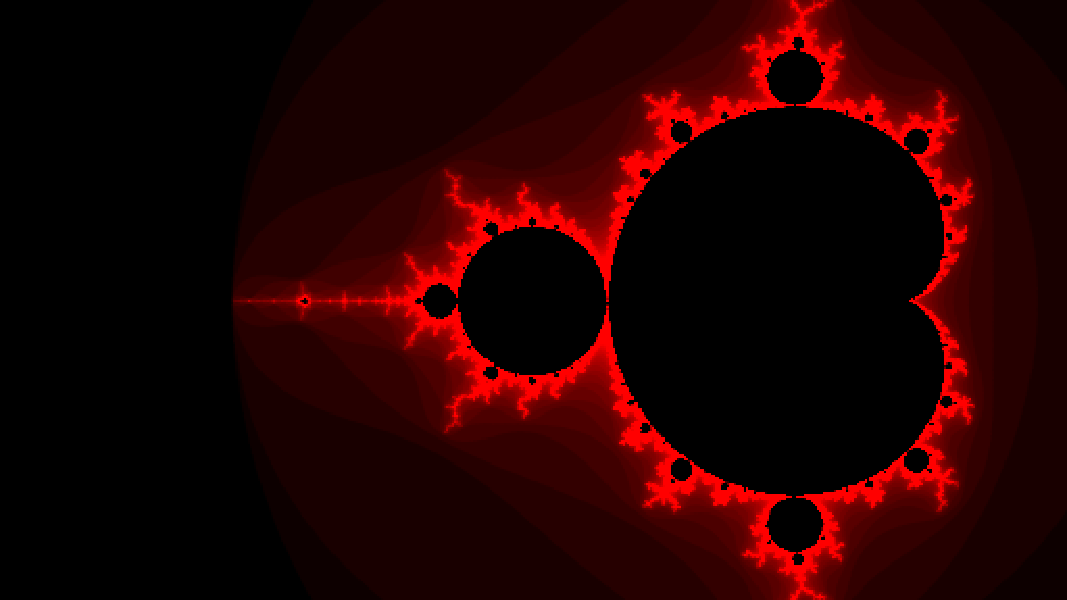
\includegraphics[width=3in, height=3in, keepaspectratio]{../img/fractal/mandelbrot.pdf}
    \caption{Mandelbrot set}
    \label{fig:mandelbrot}
 \end{center}
\end{figure}

\subsection{Distance Estimated 3D Fractals}

メンガーのスポンジ等の形状は見られたが,
マンデルブロ集合のような複雑な3次元形状を持つフラクタルが求められていた.マンデルブロ集合を3次元に拡張する試みはさまざまに行われていたものの,あまり大きな成果はあげられていなかった.例えば,ジュリア集合を4次元に拡張し,Distance Estimationを用いて描く方法が1989年には発表されている\cite{4djulia}.
しかし,その形状は単純でフラクタルコミュニティの満足のいくものではなかった.2004年にKeenan Crane氏がGPUで実装した\footnote{Ray Tracing Quaternion Julia Sets on the GPU: https://www.cs.cmu.edu/~kmcrane/Projects/QuaternionJulia/}.

2003年に発表された阿原・荒木\cite{sphairahedra}による4次元クライン群の一種であるQuasi Fuchsian 3D Fractalsはある程度の複雑性を持った3次元フラクタルであり,コミュニティに大きな影響を与えたと言われている.このフラクタルに関しては後の章で触れる.その後,2009年にマンデルブロ集合をうまく三次元に拡張したmandelbulbの出現を皮切りに,次々と複雑な三次元フラクタルの式が発見された.これらもDistance Estimationとレイマーチングを用いることで効率よくレンダリングすることができる.これら一連のフラクタルに関してはSyntopiaの一連のポスト\footnote{Syntopia Distance Estimated 3D Fractals: http://blog.hvidtfeldts.net/index.php/2011/06/distance-estimated-3d-fractals-part-i/}にまとめられている.
注意が必要なのは,これらのフラクタルは純粋な数学の研究対象になりにくい.

この章で使われている図のいくつかはFractal Lab\footnote{Fractal Lab: http://hirnsohle.de/test/fractalLab/}というWebアプリケーションを用いてレンダリングした.
\subsubsection{Mandelbulb}

mandelbulbはD.WhiteとP.Nylanderによって開発された.
White(twinbee)氏は球面座標を用いるアプローチを提案\footnote{http://www.fractalforums.com/3d-fractal-generation/true-3d-mandlebrot-type-fractal/}した.
図\ref{fig:mandelbulb2}は$z^2 + c$を用いてレンダリングした結果であるが,あまり複雑な形状は現れなかった.
しかし,その後Nylander氏が式を高次の積を扱えるように拡張した.
図\ref{fig:mandelbulb8}は$z^8 + c $という式でレンダリングされた形状であり,Mandelbulbとして広く知られている.White氏のWebページに詳しい経緯が掲載されている\footnote{http://www.skytopia.com/project/fractal/mandelbulb.html}.
レイマーチングを用いる際にはDistance Estimationを用いるが,これには通常のマンデルブロ集合で用いたものと同じアプローチを用いることができる.

\begin{figure}[h!tbp]
 \begin{subfigure}{0.49\hsize}
   \begin{center}
    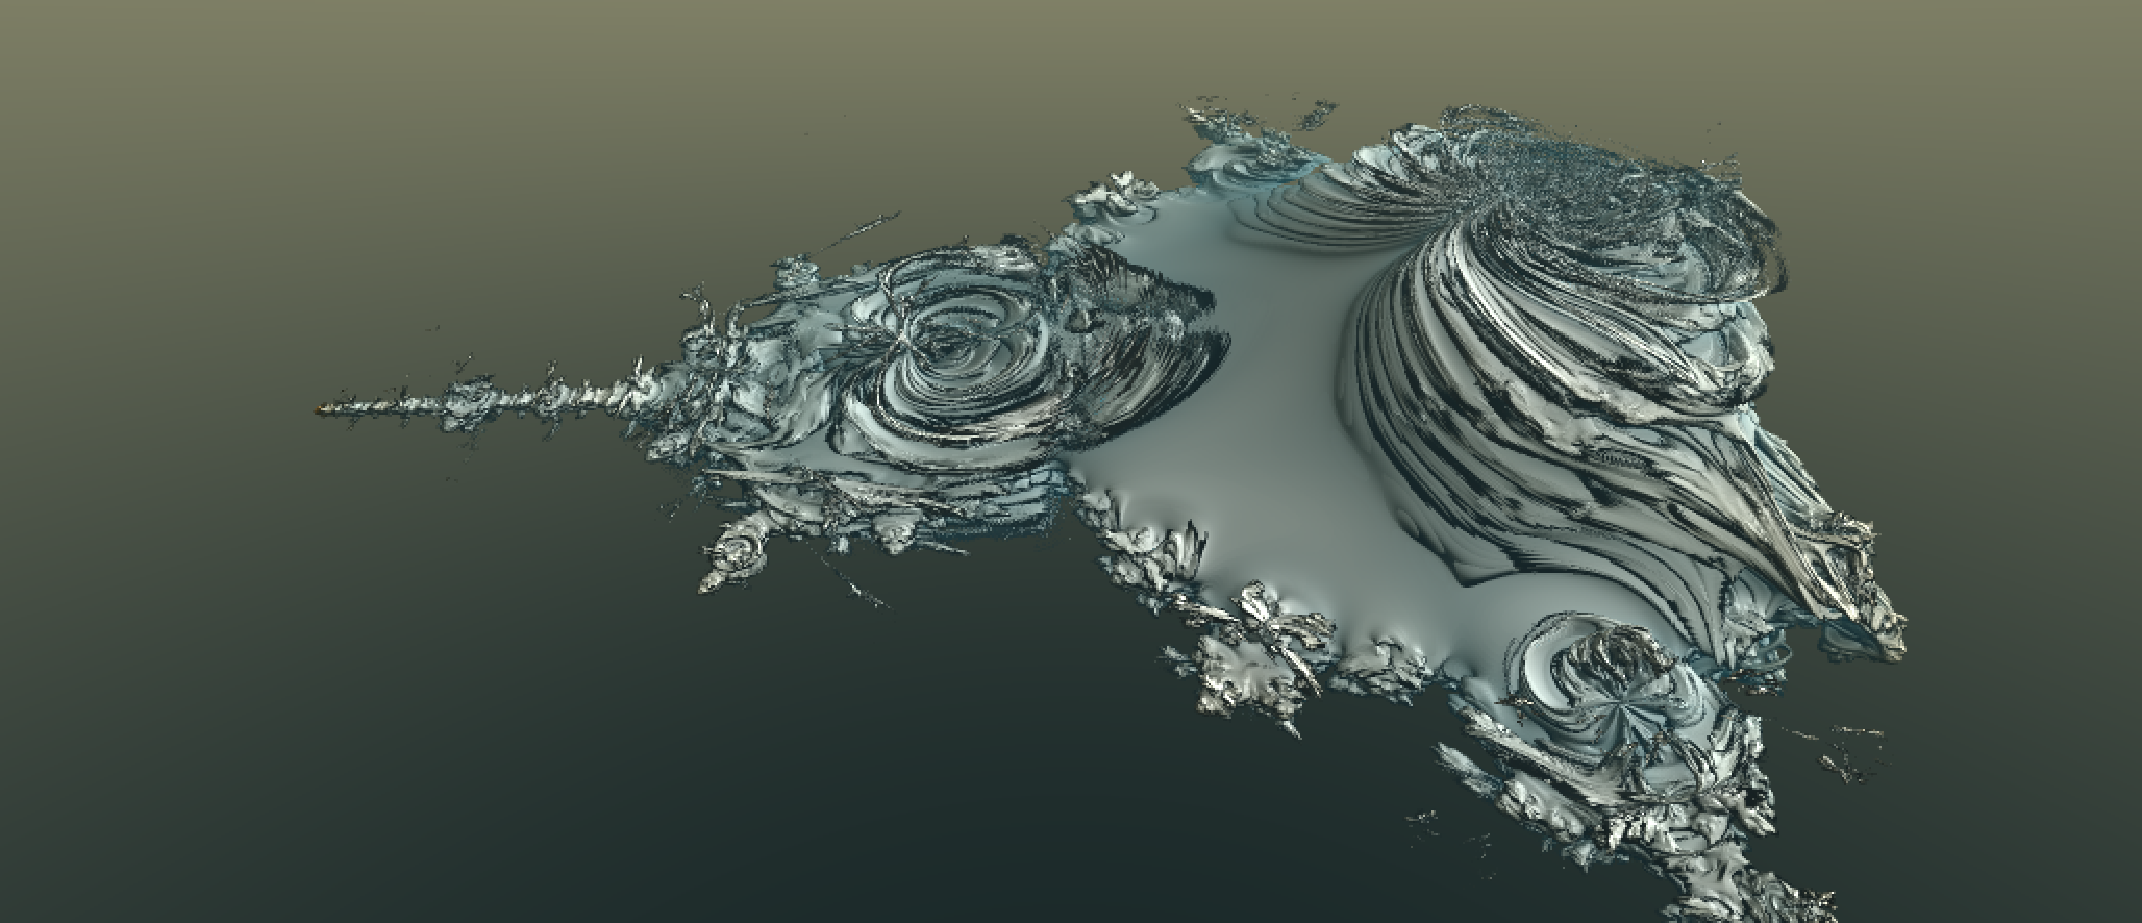
\includegraphics[width=3in, height=3in, keepaspectratio]{../img/fractal/mandelbulb2.pdf}
    \caption{$z^2 + c$}
    \label{fig:mandelbulb2}
   \end{center}
 \end{subfigure}
 \hspace*{\fill}
 \begin{subfigure}{0.49\hsize}
   \begin{center}
    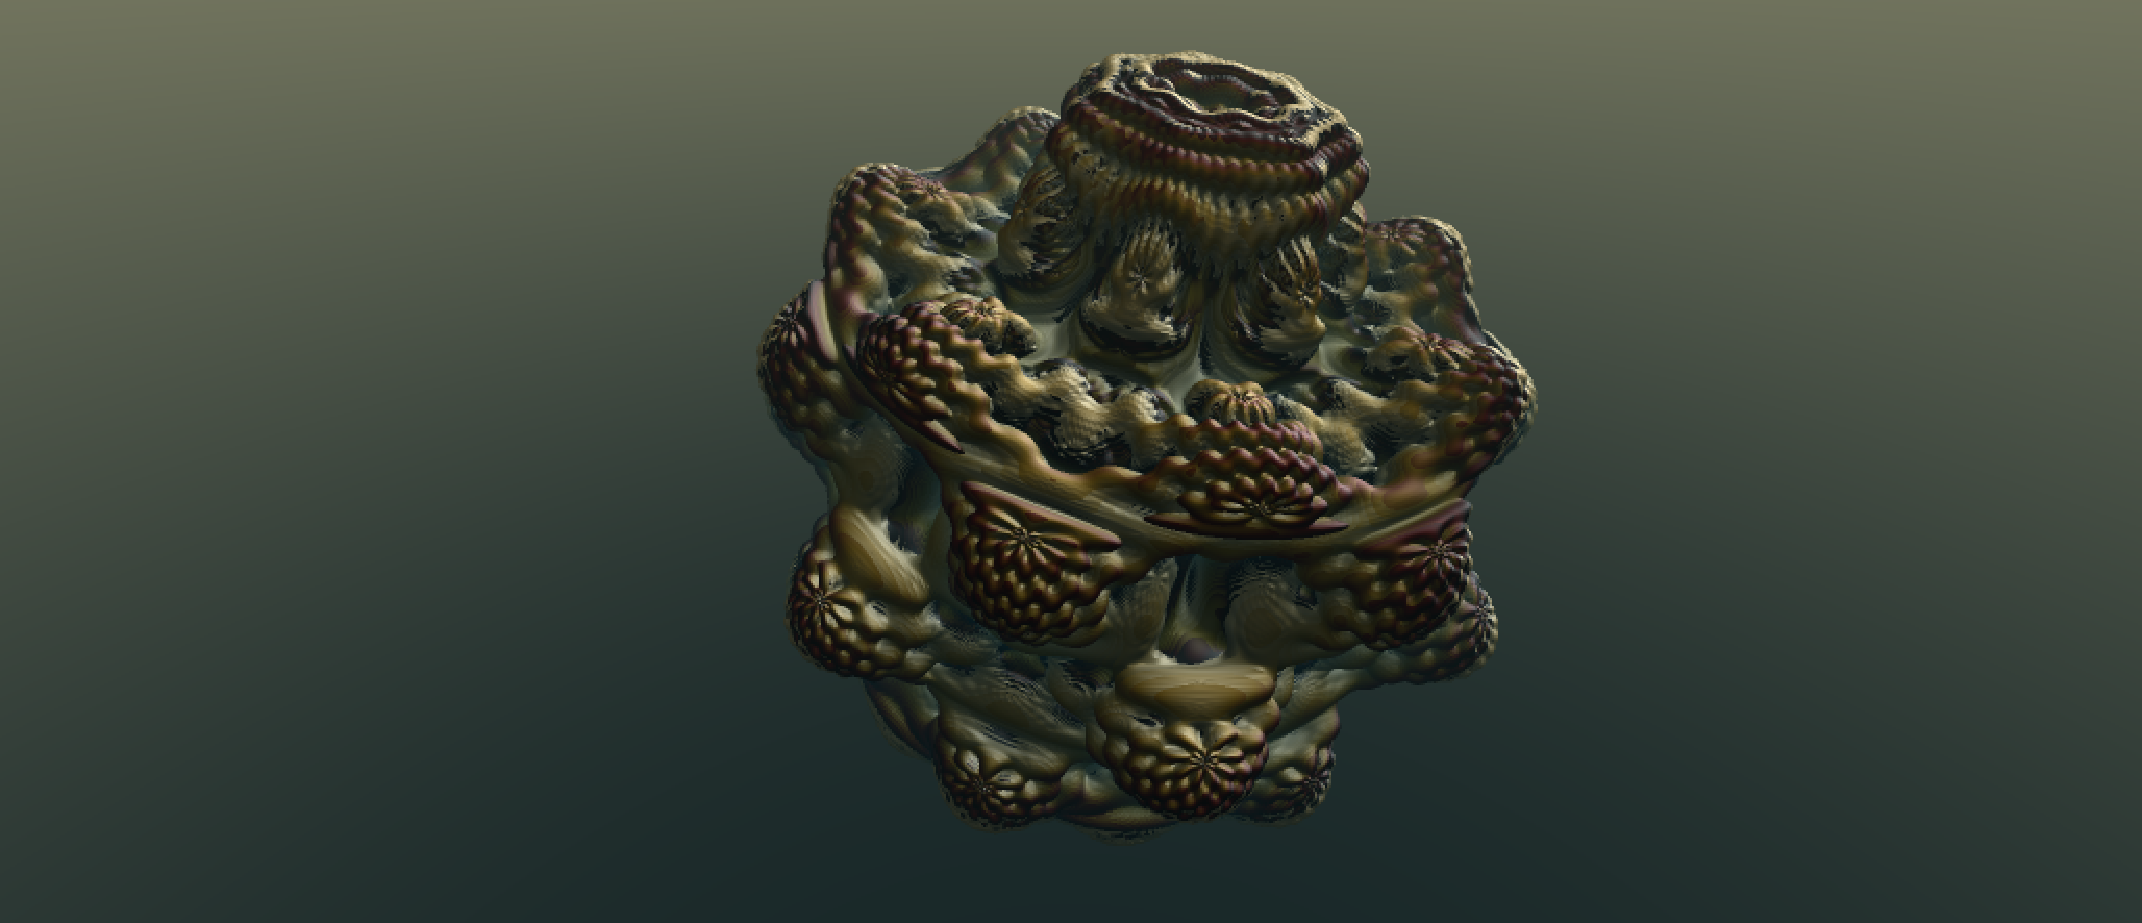
\includegraphics[width=3in, height=3in, keepaspectratio]{../img/fractal/mandelbulb8.pdf}
    \caption{$z^8 + c$}
    \label{fig:mandelbulb8}
   \end{center}
 \end{subfigure}
 \caption{Mandelbulb rendered by Fractal Lab}
\end{figure}

\subsubsection{Mandelbox}
その後,2010年にTom Lowe氏によってMandelbox\footnote{https://sites.google.com/site/mandelbox/what-is-a-mandelbox}が開発された.
Mandelboxはball foldやbox foldといった操作を定義する.
sphere foldは円の中心付近に来た点が発散してしまわないように,制限をかけた円の反転である.式は以下のように定義される.

このDistance Estimationには様々な方法があるが,mandelboxでは最終的に得られた点の原点からの距離をヤコビアンの積で割ることで距離を求めることができる.

\begin{figure}[h!tbp]
 \begin{subfigure}{0.49\hsize}
   \begin{center}
    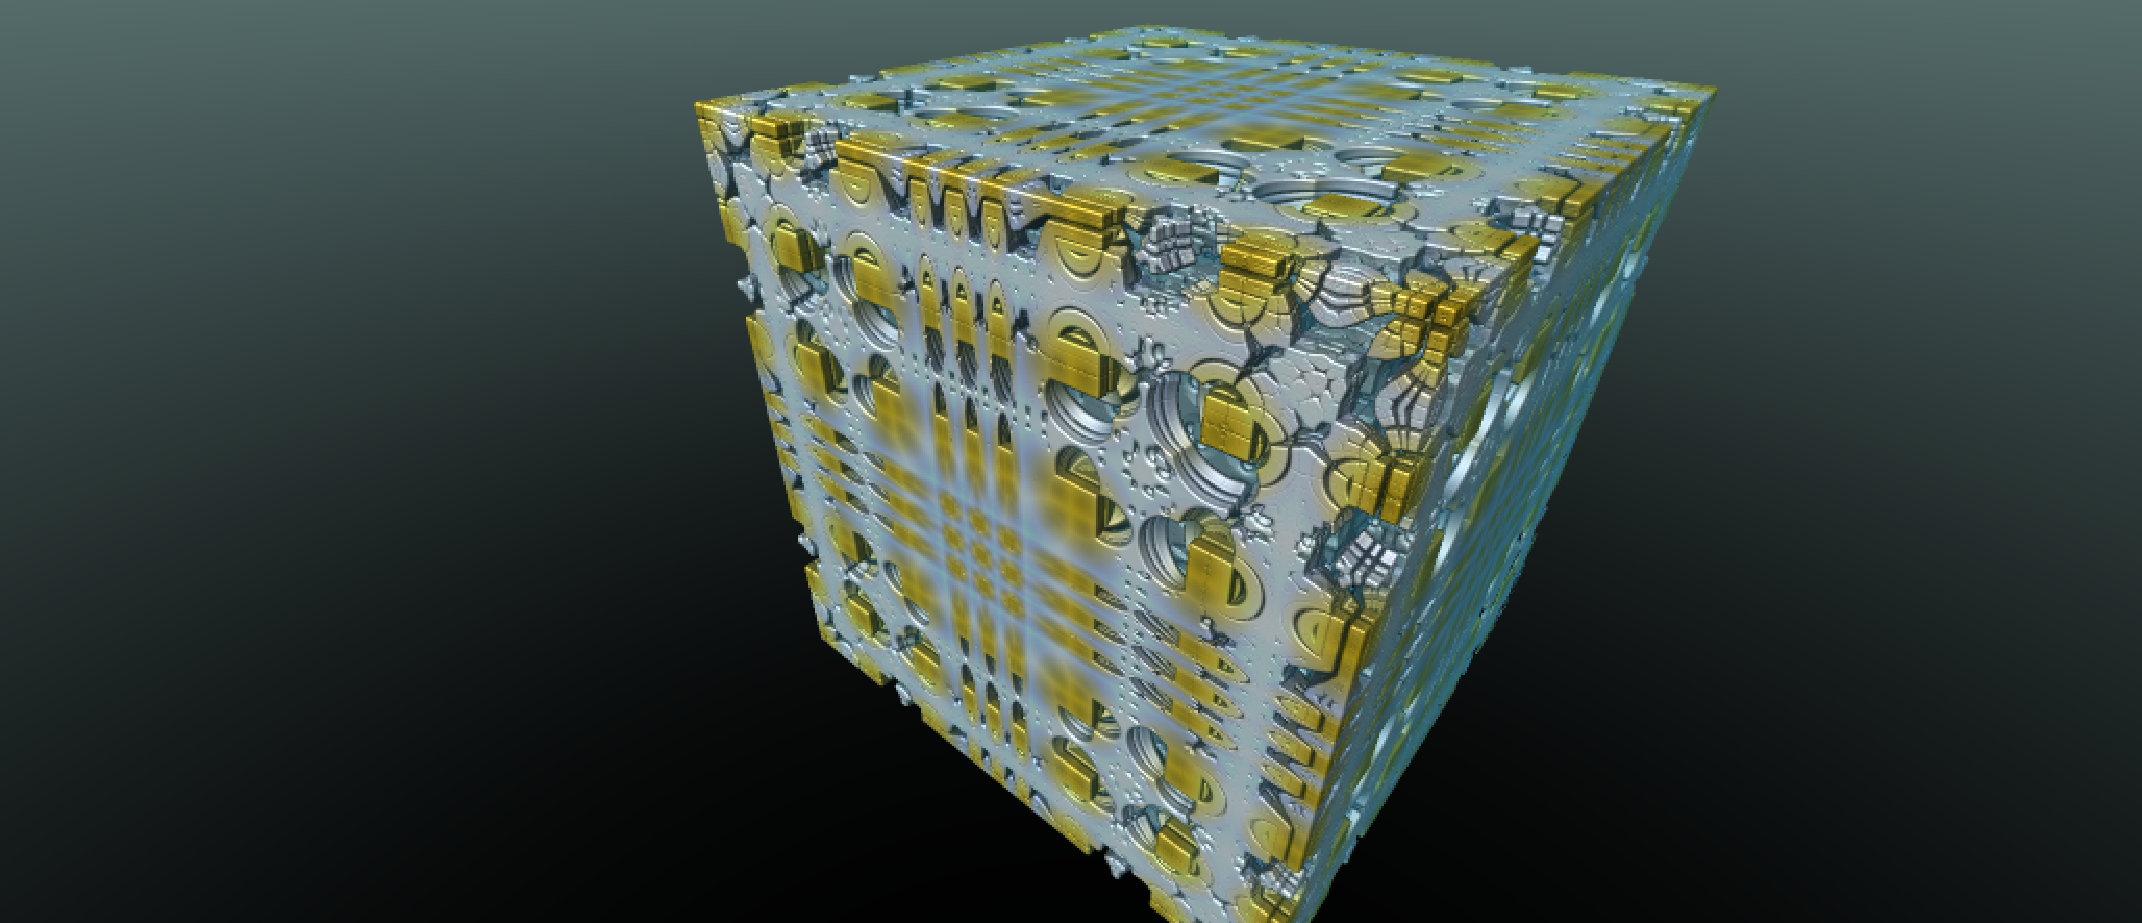
\includegraphics[width=3in, height=3in, keepaspectratio]{../img/fractal/mandelbox.pdf}
    \caption{}
    \label{fig:mandelbox}
   \end{center}
 \end{subfigure}
 \hspace*{\fill}
 \begin{subfigure}{0.49\hsize}
   \begin{center}
    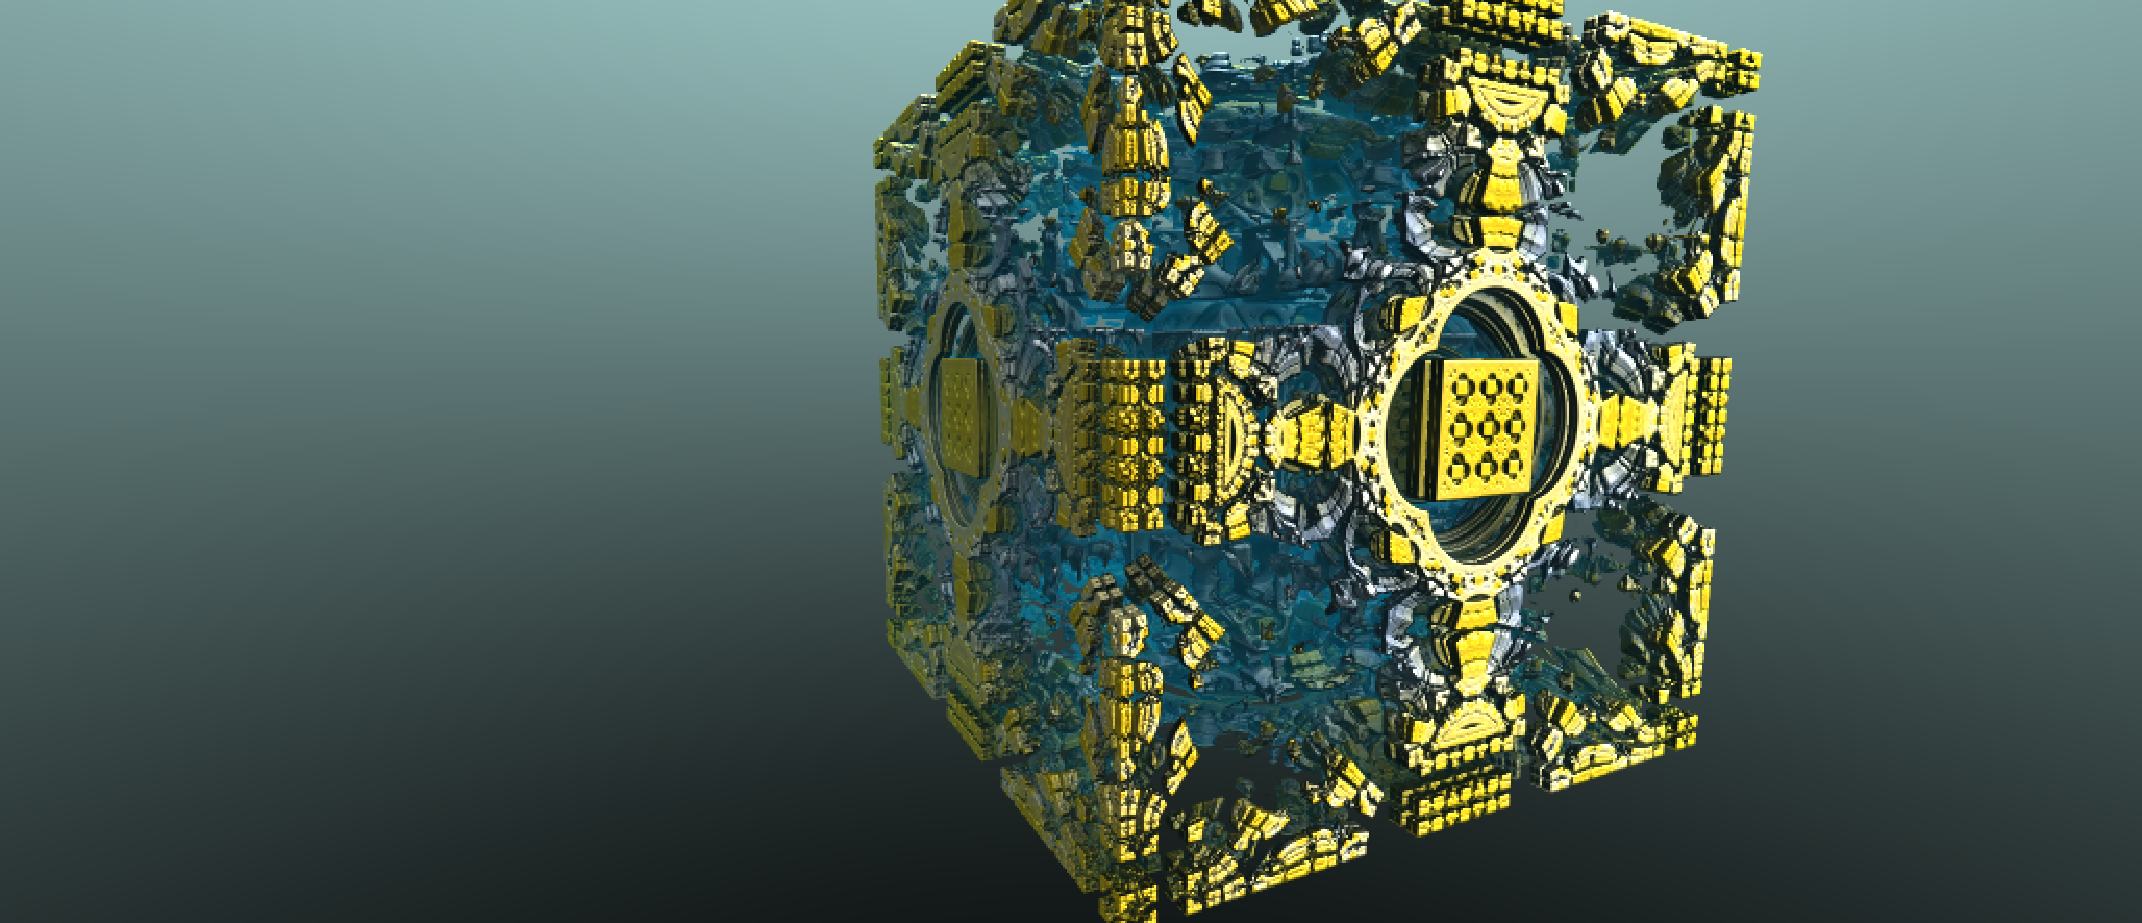
\includegraphics[width=3in, height=3in, keepaspectratio]{../img/fractal/mandelbox2.pdf}
    \caption{}
    \label{fig:mandelbox2}
   \end{center}
 \end{subfigure}
 \caption{Mandelbox rendered by Fractal Lab}
\end{figure}


\subsubsection{Pseudo-Kleinian}

mandelboxの登場以降は漸化式に複数の式を用いるHybrid Systemが考案された.今も様々なフラクタル作品が作られている.
興味深いHybrid Systemの1つにpseudo-kleinianがある.これはSpherefoldと平行移動と同じような働きをするboxfoldによってクライン群のような形状が得られる式である.

\subsection{Coloring by Orbit trap}

ここでOrbit trapと呼ばれるカラーリングのアルゴリズムを紹介しておく.Escape-timeアルゴリズムを用いたフラクタルのレンダリングでは,主にOrbit trapというカラーリングの手法が使われる.trapと呼ばれる何らかの図形を空間上に置いておき,trapと軌道の位置関係から色を付ける.
以下の図は()に点のtrapを置き,その位置に応じて色を付けた.黒の点がtrapであり,青の点が軌道である.
この方法を応用すると,画像をtrapに用いることで,図のように点の軌道上に画像を張り付けることも可能である.

\subsection{Other Fractals}

Iterated Function system(IFS)は点に様々な関数を適用して,その集積点をレンダリングするアルゴリズムである.シェルピンスキーのギャスケットなどもIFSでレンダリングすることができる.
IFSに関する書籍としてはFractals Everywhere\cite{fractalsEverywhere}が有名である.並列計算による高速化に関して以下の論文にまとめられている\cite{highPerformanceIFS}\cite{GPUIFS}.
IFSの一種にフラクタルフレーム(Fractal Frame)\cite{fractalFrame}と呼ばれるものがある.フラクタルフレームはIFSに用いる関数にメビウス変換などの非線形変換を用い,美しくレンダリングされるようにカラーリングが工夫されている.

他にも様々なアルゴリズムが存在するが,今回は後述するクライン群のレンダリングには関連してこないので触れない.Wikipedia\footnote{https://en.wikipedia.org/wiki/Fractal}には有名なアルゴリズムが網羅的に記載されているので参考にされたい.
